\chapter{More Linear Algebra}
I have wrote many pages of linear algebra theory, but that wasn't enough. So here we go, I guess.

\section{Gram–Schmidt Procedure}\label{gram}
The Gram–Schmidt procedure is a method used to produce orthonormal basis for a vectors space. For a $d$-dimensional inner product vector space $V$ with a basis vectors set $\ket{v_1}, \cdots, \ket{v_d}$, we can define a new orthonormal basis set $\{\ket{u}\}$. The first element of that set is $\ket{u_1} = \ket{v_1}/\norm{\ket{v_1}}$, with the following element $\ket{v_{k+1}}$  being:
$$
\ket{u_{k+1}} = \frac{\ket{v_{k+1}} - \sum_{i=1}^{k} \bra{u_i}\ket{v_{k+1}}\ket{u_i}}{\norm{\ket{v_{k+1}} - \sum_{i=1}^{k} \bra{u_i}\ket{v_{k+1}}\ket{u_i}}}
$$
For $k$ in the interval $1 \leq k \leq d-1$.

If we follow the above for each $k$ in $1 \leq k \leq d-1$, we obtain the new vector set $\ket{u_1}, \cdots , \ket{u_d}$ that is a valid orthonormal basis for the space $V$. The created vector set must have the same span\footnote{The span of a set of vectors is all the possible linear combinations that come from those vectors.} as the previous one to be a valid basis for the space $V$:
$$
\text{span}(\{\ket{v}\}) = \text{span}(\{\ket{v}\}) = V
$$
Note that the span of the basis set is the definition of the space. In other words, every vector in $V$ can be represented as a linear combination of the basis vectors. 

To get at some intuition let's look at the case for $k=1$:
$$
\ket{u_2} = \frac{\ket{v_2} - \bra{u_1}\ket{v_2}\ket{u_1}}{\norm{\ket{v_2} - \bra{u_1}\ket{v_2}\ket{u_1}}}
$$
We can see that the vector $\ket{u_2}$ is defined by the subtraction of the vector $\ket{v_2}$ by the projection\footnote{The way to project the vector $\ket{a}$ onto $\ket{b}$ is: $\bra{b}\ket{a}\ket{b}$.} of $\ket{v_2}$ onto $\ket{v_1}$. Which is equivalent for the projection of $\ket{v_2}$ onto $\ket{u_1}$, remember that $\ket{u_1}$ is just $\ket{v_1}$ normalized. Therefore we have: 
\begin{figure}
	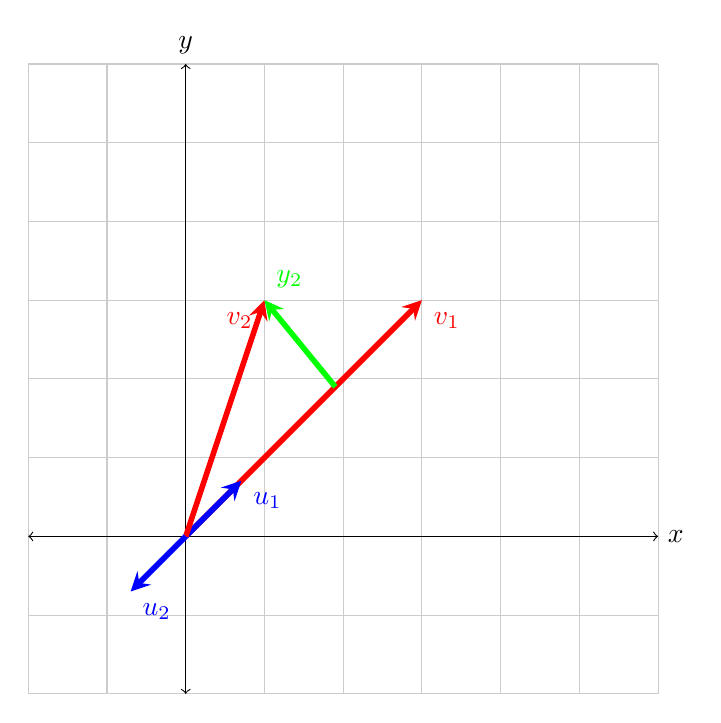
\begin{tikzpicture}
		\draw[thin,gray!40] (-2,-2) grid (6,6);
		\draw[<->] (-2,0)--(6,0) node[right]{$x$};
		\draw[<->] (0,-2)--(0,6) node[above]{$y$};
		\draw[line width=2pt,red,-stealth](0,0)--(3,3) node[anchor=north west]{$\boldsymbol{\ket{v_1}}$};
		\draw[line width=2pt,blue,-stealth](0,0)--(0.7071,0.7071) node[anchor=north west]{$\boldsymbol{\ket{u_1}}$};
		\draw[line width=2pt,red,-stealth](0,0)--(1,3) node[anchor=north east]{$\boldsymbol{\ket{v_2}}$};
		\draw[line width=2pt,green,-stealth](1.9,1.9)--(1,3) node[anchor=south west]{$\boldsymbol{\ket{y_2}}$};
		\draw[line width=2pt,blue,-stealth](0,0)--(-0.7,-0.7) node[anchor=north west]{$\boldsymbol{\ket{u_2}}$};
	\end{tikzpicture}
\end{figure}


The proof that is an orthonormal basis is quite simple: 
We can see immediately that the components of $\{ \ket{u} \}$ are unit vectors because they are normalized (the vectors $\ket{v_{k+1}} - \sum_{i=1}^{k} \bra{u_i}\ket{v_{k+1}}\ket{u_i}$ are divided by their norm). And we can se that they are orthogonal by checking that the inner product of non-equal vectors in the set is 0: 

For $k=1$:
$$
\ket{u_2} = \frac{\ket{v_2} - \bra{u_1}\ket{v_2}\ket{u_1}}{\norm{\ket{v_2} - \bra{u_1}\ket{v_2}\ket{u_1}}}
$$
Then the inner product with $\ket{v_1}$ is:
$$
\begin{aligned}
\bra{u_1}\ket{u_2} 
&= \bra{u_1} \left( \frac{\ket{v_2} - \bra{u_1}\ket{v_2}\ket{u_1}}{\norm{\ket{v_2} - \bra{u_1}\ket{v_2}\ket{u_1}}} \right) \\
&= \frac{\bra{u_1}\ket{v_2} - \bra{u_1}\ket{v_2}\bra{u_1}\ket{u_1}}{\norm{\ket{v_2} - \bra{u_1}\ket{v_2}\ket{u_1}}} \\
&= 0
\end{aligned}
$$
By induction we can see that for $j \leq d$, with $d$ being the dimension of the vector space:
$$
\begin{aligned}
	\bra{u_j}\ket{u_{n+1}} 
	& = \bra{u_j} \left( \frac{\ket{v_{n+1}} - \sum_{i=1}^{n} \bra{u_i}\ket{v_{n+1}}\ket{u_i}}{\norm{\ket{v_{n+1}} - \sum_{i=1}^{n} \bra{u_i}\ket{v_{n+1}}\ket{u_i}}} \right) \\
	& = \frac{\bra{u_j}\ket{v_{n+1}} - \sum_{i=1}^{n} \bra{u_i}\ket{v_{n+1}} \bra{u_j}\ket{u_i}}{\norm{\ket{v_{n+1}} - \sum_{i=1}^{n} \bra{u_i}\ket{v_{n+1}} \ket{u_i}}} \\
	& = \frac{\bra{u_j}\ket{v_{n+1}} - \sum_{i=1}^{n} \bra{u_i}\ket{v_{n+1}} \delta_{ij}}{\norm{\ket{v_{n+1}} - \sum_{i=1}^{n} \bra{u_i}\ket{v_{n+1}} \ket{u_i}}} \\
	& = \frac{\bra{u_j}\ket{v_{n+1}} - \bra{u_j}\ket{v_{n+1}}}{\norm{\ket{v_{n+1}} - \sum_{i=1}^{n} \bra{u_i}\ket{v_{n+1}} \ket{u_i}}} \\
	& = 0	\\
\end{aligned}
$$
All of this doesn't seem straightforward at first but remember that the inner product of two orthogonal vectors is zero, and the inner product between the same unit vector is one. 

\section{Dirac Notation Crash Course}

On the following table there is a quick summary important mathematical concepts of linear algebra expressed in Dirac Notation\footnote{The notation used for the complex vector spaces and complex number space are not standard Dirac Notation, but I included them in the table to explain what they mean.}. 
%Along the text you may encounter more complicated use of this notation. 

\begin{tabular}{ p{2cm}|p{12cm} }
	\hline
	Notation & Description \\
	\hline
	\hline
	$z$ & Complex number    \\
	$z^{*}$ & Complex conjugate of the a complex number $z$. $(a+ bi)^{*} = (a -bi)$\\
	$\ket{\psi} $ & Vector with label $\psi$. Known as \textit{ket}\\
	$\ket{\psi}^T$ & Transpose of vector $\ket{\psi}$ \\
	$\ket{\psi}^\dag $ &  Hermitian conjugate of vector. $\ket{\psi}^\dag = (\ket{\psi}^T)^* $\\
	$\bra{\psi} $ & Dual vector to $\ket{\psi}$. $ \ket{\psi} = \bra{\psi}^{\dag}$ and $\bra{\psi} = \ket{\psi}^\dag$. Known as \textit{bra}\\
	$ \bra{\varphi}\ket{\psi} $ & Inner product of vectors $\bra{\varphi}$ and $\ket{\psi}$ \\
	$ \ket{\varphi}\bra{\psi} $ & Outer product of vectors $\bra{\varphi}$ and $\ket{\psi}$ \\
	$ \ket{\psi}\otimes\ket{\varphi}$ & Tensor product of vectors $\ket{\varphi}$ and $\ket{\psi}$ \\
	$ 0 $ & Zero vector and zero operator \\
	$ \mathbb{I}_n $ & Identity matrix of dimension $n$ \\
	$ \mathbb{C}_n $ & Complex vector space of dimension $n$ \\
	$ \mathbb{C}_1$ or $\mathbb{C} $ & Complex number space \\
	
\end{tabular}
\section{More on the Partial Trace}

\chapter{Quantum Computation vs Quantum Mechanics}
On the introduction I mentioned that one of the reasons for with I started learning and researching quantum computing is because it is easy, on this appendix I am going to present why this is the case with a practical example.

On quantum mechanics the more general way to represent quantum state, like the orbitals of an atom of hydrogen, are wavefunctions, not statevectors. Wavefunctions are extremely useful, however, working with them adds a hole new level of complexity because they are continuous functions that are dependent on time. Compare them with vectors, which are discrete packets of information that evolve through discrete amounts of time.

\section{Normalizing}
Because the probabilistic interpretation of both statevectors and wavefunctions, these two objects have to be normalize upon measurement, thus making the total sum of probabilities $1$. How to normalize these objects is a perfect example to illustrate the difference in complexity that I see between quantum mechanics and quantum computation. 

They way to get compute the probabilities of a measurement out of a wavefunctions is by squared it. For a wavefunction $\Psi$ that represents a particle, the probability of finding the particle in a point $x$ is $\abs{\Psi(x,t)}^2$. Then, the wavefunction has to be normalized like the following:
$$
\int_{-\infty}^{+\infty}\abs{\Psi(x,t)}^2\, dx\ = 1
$$

\chapter{Polarization of a photon}
\label{appendix:optics}
On equation \ref{eq:photon_state} I have excluded the concept of phase, which determinates the type of polarization that the photon has. There are three types of polarization:
\begin{enumerate}
	\item \textbf{Linear:}
	A photon is linear polarized when the phase angles $\alpha_x$, $\alpha_y$ of both basis $\ket{x},\ket{y}$ states are equal:
	\begin{align*}
		\ket{\nearrow} &= \cos\theta\exp(i\alpha_x)\ket{x} + \cos\theta\exp(i\alpha_y)\ket{y} \\
		&= [\cos\theta\ket{x} + \sin\theta\ket{y}]\exp(i\alpha)
	\end{align*}
	Where $\alpha=\alpha_x=\alpha_y$.
	
	\item \textbf{Circular:}
	Where the angles $\alpha_x$, $\alpha_y$ are apart exactly $\frac{\pi}{2}$ and the amplitude of both basis states is the same:
	\begin{align*}
		\ket{\nearrow} &= \frac{1}{\sqrt{2}}\cos\theta\exp(i\alpha_x)\ket{x} \pm i\frac{1}{\sqrt{2}}\sin\theta\exp(i\alpha_y)\ket{y} \\
					   &= [\cos\theta\exp(i\alpha_x)\ket{x} \pm i\sin\theta\exp(i\alpha_y)\ket{y}]\frac{1}{\sqrt{2}}
	\end{align*}
Where the $\pm$ sign indicates the difference between right and left circular polarization, $+$ and $-$, respectively. 

	\item \textbf{Elliptical:}
	Where just the phase angles $\alpha_x$, $\alpha_y$ differ in some amount:
	$$
	\ket{\nearrow} = \cos\theta\exp(i\alpha_x)\ket{x} + \cos\theta\exp(i\alpha_y)\ket{y}
	$$
	This is the more general case.
	
\end{enumerate}